\section{Methodology}
\label{sec:methodology}

\begin{figure*}[h!]
	\centering
	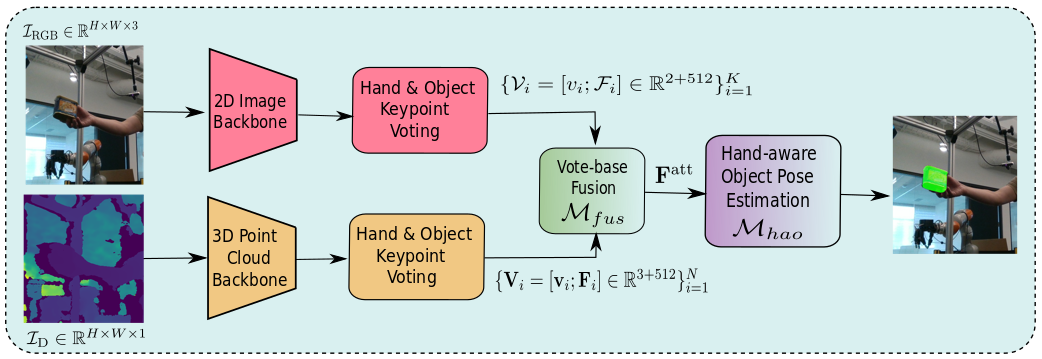
\includegraphics[width=0.98\linewidth]{figs/overview}
	\caption{Overview of our proposed framework for estimating the 6D pose of hand-held objects from RGB-D images. The framework comprises several key components: (1) feature extraction backbones for both 2D images and 3D point clouds, which process the RGB and depth information, respectively; (2) voting modules that generate votes for keypoint locations in both 2D and 3D spaces; (3) a vote-based fusion module $\mathcal{M}_{fus}$ that effectively combines the multimodal data to address the challenges of occlusions and representation distribution shifts; and (4) a hand-aware object pose estimation module $\mathcal{M}_{hao}$, which models the interactions between the hand and the object using a self-attention mechanism.}
	\label{fig:overview}
\end{figure*}

Our objective is to determine the 6D pose of a hand-held object within an RGB-D image. We assume the availability of an accurate 3D model of the object, with its coordinate system $\mathcal{O}$ defined in the model's 3D space. The pose of the object is described by a rigid transformation from the object coordinate system to the camera coordinate system $\mathcal{G}$. This transformation comprises a rotation matrix $R \in SO(3)$ and a translation vector $t \in \mathbb{R}^{3}$, collectively represented as $\xi = [R|t]$. Figure \ref{fig:overview} illustrates the overall pipeline of our framework. Our network consists of backbones for extracting features from both 2D images and 3D point clouds, voting modules, a vote-based fusion module $\mathcal{M}_{fus}$, and a hand-aware object pose estimation module $\mathcal{M}_{hao}$.

\subsection{3D Point Cloud Branch}

Given a depth image, the 3D point cloud branch network converts the image to a 3D point cloud and proceeds to cast votes for 3D keypoints of both hand and objects. Inspired by VoteNet (\cite{qi2019deep}), wherein 3D points participate in voting for object centers in object detection tasks, we have formulated our network to predict keypoint locations for individual 3D points. Specifically, we utilize the PointNet++ architecture (\cite{qi2017pointnet++}) with multi-scale grouping as our backbone network to extract geometric features. The backbone network takes $N$ points as input and enriches them with high-dimensional features $\{\mathbf{p}_{i}\}_{i=1}^{N}$ where $\mathbf{p}_{i} = [\mathbf{x}_i; \mathbf{f}_i]$ with $\mathbf{x}_{i}\in\mathbb{R}^{3}$ being the point location in 3D space and $\mathbf{f}_{i} \in \mathbb{R}^{512}$ being a feature vector.

Subsequently, the points $\{\mathbf{p}_{i}\}_{i=1}^{N}$ are fed into a multi-layer perceptron (MLP) to compute votes $\{\mathbf{V}_{i} = [\mathbf{v}_{i}; \mathbf{F}_{i}] \in \mathbb{R}^{3+512} \}_{i=1}^{N}$. The MLP consists of four fully connected layers, ReLU and batch normalization. Each vote $\mathbf{V}_i$ is represented by a point $\mathbf{v}_{i}$ in 3D space with its Euclidean coordinates supervised to be close to a keypoint $\mathbf{s}_i$, and a feature vector $\mathbf{F}_{i}$. To supervise the learning of votes $\{\mathbf{V}_{i} = [\mathbf{v}_{i}; \mathbf{F}_{i}] \in \mathbb{R}^{3+512} \}_{i=1}^{N}$, we apply a regression loss:

\begin{equation}
L_{\text{3d-vote}} = \dfrac{1}{N_{oh}} \sum_{i}  \| \mathbf{v}_{i} - \hat{\mathbf{v}}_{i} \|_{H} \cdot \mathds{1}(\mathbf{v}_{i})
\end{equation}

\noindent Here, $N_{oh}$ is the count of the total number of points on the object and hand, $\hat{\mathbf{v}}_{i}$ is the location of the closest ground truth keypoint, $\parallel\cdot\parallel_{H}$ is the Huber norm and $\mathds{1}(\cdot)$ is a binary function indicating whether the point $\mathbf{p}_i$ belongs to the hand or object. At this stage, we have a set of votes $\{\mathbf{V}_i = [\mathbf{v}_i; \mathbf{F}_i] \in \mathbb{R}^{3+512}\}_{i=1}^{N}$.

\subsection{2D Image Branch}

Given an input color image, this network branch predicts hand and object 2D keypoints. We adopt a pixel-wise direction prediction strategy, which encourages the network to prioritize local hand and object characteristics while minimizing the influence of cluttered backgrounds. We employ ResNet-34 (blocks 1, 2, 3, and 4) as the encoder, coupled with four up-sampling layers serving as the decoder (\cite{he2016deep}). The upsampling layers consist of transposed convolutional layers with batch normalization and ReLU activation. For a given pixel $p$, the network predicts a scale-invariant vector $\hat{\mathfrak{u}}(p)$, representing the direction from pixel $p$ to the closest keypoint $s$.

\begin{equation} 
\hat{\mathbf{u}}(p) = \frac{s - p}{\parallel s - p \parallel_2}
\end{equation}

\noindent To supervise the learning of unit vectors, we apply a smooth $L_1$ loss, similar to the approach in \cite{girshick2015fast}. The loss function $L_{\text{2d-vote}}$ is defined as:

\begin{equation} 
L_{\text{2d-vote}} = \dfrac{1}{N_{oh}} \sum_{p \in (\mathcal{O} \cup \mathcal{H})} \text{smooth}_{L_1} ( \hat{\mathbf{u}}(p) - \mathbf{u}(p) )
\end{equation}

\noindent Here, $N_{oh}$ is the count of the total number of pixels on the object and hand. $\mathbf{u}$ denotes the predicted vector, $\hat{\mathbf{u}}$ represents the ground truth unit vector, and $p \in (\mathcal{O} \cup \mathcal{H})$ indicates that pixel $p$ pertains to hand or object. Votes are generated by randomly selecting two pixels situated within a specific radius and then calculating the intersection of their respective vectors. Additionally, a representative feature is computed for these selected pixels through feature concatenation. This process is iterated $K$ times, leading to the generation of votes $\{ \mathcal{V}_{i} = [v_i; \mathcal{F}_i] \in \mathbb{R}^{2+512} \}_{i=1}^{K}$. $v_i \in \mathbb{R}^2$ represents the 2D vote location, and $\mathcal{F}_i \in \mathbb{R}^{512}$ represents the high-dimensional feature of the vote $v_i$.

\subsection{Vote-based Feature Fusion}

Given the votes \(\{\mathbf{V}_i = [\mathbf{v}_i; \mathbf{F}_i] \in \mathbb{R}^{3+512}\}_{i=1}^{N}\) from the 3D branch and \(\{\mathcal{V}_i = [v_i; \mathcal{F}_i] \in \mathbb{R}^{2+512}\}_{i=1}^{K}\) from the 2D branch, we perform vote-based fusion using a channel attention mechanism adapted for 3D data. For each geometric vote feature \(\mathbf{F}_i\) paired with its 3D point coordinate \(\mathbf{v}_i\), we retrieve the corresponding visual vote features from \(\mathcal{F}\) by projecting its neighborhood within a radius \(r\) onto the image plane. We then sample the \(k\) nearest neighbor votes within this region to gather their visual features. If fewer than \(k\) pixels exist in the corresponding region, null features are padded. The collected visual features are integrated using max pooling and processed through Multi-Layer Perceptrons (MLPs) to align their channel size with that of the point cloud features, producing modified visual vote features \(\mathcal{F}^{'}\):

\[
\mathcal{F}_i^{\text{proj}} = \text{MaxPool}(\{\mathcal{F}_j \mid \| v_j - \mathbf{v}_i \|_2 < r \})
\]

\[
\mathcal{F}_i^{'} = \text{MLP}_{\text{match}}(\mathcal{F}_i^{\text{proj}})
\]

\noindent Next, these integrated visual vote features \(\mathcal{F}_i^{'}\) are concatenated with the geometric vote features \(\mathbf{F}_i\), and a shared MLP is applied to produce fused vote features \(\{\mathbf{V}_i = [\mathbf{v}_i; \mathbf{F}_i^{\text{fus}}] \in \mathbb{R}^{3+1024}\}_{i=1}^{N}\):

\[
\mathbf{F}_i^{\text{fus}} = \text{MLP}_{\text{shared}}([\mathbf{F}_i; \mathcal{F}_i^{'}])
\]

\noindent To enhance these fused features, we employ a 3D channel attention module. This module uses global average pooling across all votes to generate a channel descriptor for each feature map. Specifically, global average pooling compresses each channel by computing the average of all values in that channel across all votes, resulting in a descriptor vector \(\mathbf{z}_c\):

\[
\mathbf{z}_c = \frac{1}{N} \sum_{i=1}^{N} \mathbf{F}^{\text{fus}}_i
\]

\noindent The channel descriptors are then passed through two fully connected layers to learn a weight vector. The first fully connected layer reduces the dimensionality, and the second fully connected layer restores it back to the original number of channels. Both layers use ReLU activations, except the final layer, which uses a sigmoid activation to normalize the weights between 0 and 1:

\[
\mathbf{w} = \sigma(\text{FC}_2(\text{ReLU}(\text{FC}_1(\mathbf{z}))))
\]

\noindent where \(\sigma\) denotes the sigmoid activation function. The learned weights are used to scale the channels of the fused feature map, effectively emphasizing the most informative channels and suppressing the less relevant ones:

\[
\mathbf{F}_i^{\text{att}} = \mathbf{w} \odot \mathbf{F}_i^{\text{fus}}
\]

\noindent where \(\odot\) denotes the Hadamard product (element-wise multiplication). This attention-enhanced fused feature, \(\mathbf{F}_i^{\text{att}}\), leverages both the geometric and visual information for improved hand-held object pose estimation. The channel attention mechanism recalibrates the features in each channel of the original feature points, enhancing the representation of more informative channels and suppressing less relevant ones. The design of this vote-based feature fusion is well-suited for RGB-D data fusion. By combining 2D and 3D features, we leverage the texture and color of RGB images with the spatial details of depth data. The radius-based neighborhood projection keeps the integration locally relevant, capturing necessary fine-grained details. Additionally, the channel attention mechanism enhances the fused features by prioritizing the most informative channels, reducing noise and redundancy, and dynamically adjusting each channel's contribution based on its relevance.

\subsection{Hand-aware Object Pose Estimation}

Given a set of votes $\{\mathbf{V}_i = [\mathbf{v}_i; \mathbf{F}_i^{\text{att}}] \in \mathbb{R}^{3+512}\}_{i=1}^{N}$, we sample a subset of $M$ votes (where $M < N$) using farthest point sampling based on $\{\mathbf{v}_i\}$ in 3D Euclidean space, to get $\{\mathbf{v}_i^m\}$ with $m = 1, \ldots, M$. Then we form $M$ clusters by finding neighboring votes to each of the $\mathbf{v}_i^m$'s 3D location:
\[
\mathbf{C}_m = \{\mathbf{V}_i \mid \|\mathbf{v}_i - \mathbf{v}_i^m\| \leq r\} \quad \text{for} \ m = 1, \ldots, M
\]
Here, $\mathbf{C}_m$ is the set of votes in the $m$-th cluster. Votes from each cluster are independently processed by $\text{MLP}_1$ before being max-pooled (channel-wise) to a single feature vector and passed to $\text{MLP}_2$ where information from different votes is further combined. Finally, each cluster yields a keypoint with a 3D position $\mathbf{x}_{j}^{\text{kp}} \in \mathbb{R}^{3}$ and an aggregated feature vector $F_{i} \in \mathbb{R}^{512}$. 

To better learn the relationship between the hand and the object, we integrate a self-attention module into the keypoint feature learning process. This module, inspired by the self-attention mechanism (\cite{zhang2019self}), encodes meaningful spatial relationships between the keypoints' features. Given the aggregated features $\{F_i \in \mathbb{R}^{512}\}_{i=1}^M$ from the $M$ keypoints, we apply the self-attention mechanism as follows. Firstly, the feature map $F_i$ is fed into two MLPs to generate two new feature maps $X$ and $Y$:
\[
X = \text{MLP}_1(F_i)
\]
\[
Y = \text{MLP}_2(F_i)
\]
Next, the attention map $W$ is computed as:
\[
W_{j,i} = \frac{\exp(Y_j \cdot X_i^T)}{\sum_{i=1}^{M} \exp(Y_j \cdot X_i^T)}
\]
where $W_{j,i}$ indicates that the $i$-th keypoint impacts the $j$-th keypoint. The original feature map $F_i$ is then fed into another MLP to output a new feature map $Z$:
\[
Z = \text{MLP}_3(F_i)
\]
We multiply $Z$ with the transpose of $W$ to generate the aggregated features $A^P$:
\[
A^P = W^T Z
\]
We then add a scale parameter $\mu$ and the original features to obtain the final enhanced feature map $F_i^{\text{att}}$:
\[
F_i^{\text{e}} = \mu A^P + F_i = \mu W^T Z + F_i
\]

This self-attention mechanism allows the network to learn the dependencies between different keypoints, capturing the complex relationships between the hand and the object, thus enhancing the feature representation for the hand-held object pose estimation. By incorporating this self-attention mechanism, the model can effectively leverage the spatial relationships between the keypoints to improve the accuracy and robustness of the pose estimation, leading to a more precise understanding of the hand-object interaction.

Given the enhanced keypoint features $\{\mathbf{F}_i^{\text{e}} \in \mathbb{R}^{512}\}_{i=1}^M$, we proceed to regress the object pose. Each enhanced feature $\mathbf{F}_i^{\text{e}}$ is input into an MLP-based regression network to predict the 3D object pose parameters. This regression network consists of several fully connected layers with ReLU activations, followed by an output layer that predicts the translation vector $\mathbf{t} \in \mathbb{R}^{3}$ and the rotation quaternion $\mathbf{q} \in \mathbb{R}^{4}$. The predicted pose $\{\mathbf{t}, \mathbf{q}\}$ represents the 3D translation and rotation of the object relative to the hand.

To train the network, we jointly supervise the learning of our modules using a multi-task loss function. This multi-task loss integrates several task-specific losses, each weighted by a respective factor, to ensure a balanced learning process across different aspects of pose estimation.

\begin{align}
L = L_{pose} + L_{3d-vote} + L_{2d-vote} + L_{sem}
\label{eq:loss}
\end{align}

\noindent Here, \(L\) represents the total loss, composed of the pose loss (\(L_{pose}\)), 3D voting loss (\(L_{3d-vote}\)), 2D voting loss (\(L_{2d-vote}\)), and semantic classification loss (\(L_{sem}\)). Following \cite{wang2019densefusion}, the pose loss is calculated as the distance between points sampled on the object model in the ground truth pose and the corresponding points transformed by the predicted pose. For symmetric objects, we minimize the distance from each point on the predicted model orientation to the nearest point on the ground truth model.